
% \chapter{$^{162}$DY RESULTS AND DISCUSSION}

\section{$^{162}$Dy Lifetimes}



In the remaining level schemes in Chapter 5, the widths of transitions are proportional to the calculated reduced transition probabilities for a particular $\gamma$-ray and are scaled and normalized to guide the eye; for example, a 1~mW.u. B(E1) is approximately equal in width to a 5~W.u. B(E2) transition strength and $\sim$0.1~W.u. for a B(M1), unless otherwise noted in a particular section of discussion. This scaling is in line with the understanding that enhanced E1 transitions are $\sim$1~mW.u., large E2 transition strengths are $>$5~W.u., and inflated M1 transitions are $\sim$0.1~W.u. in strength. To further aid the eye, E1, E2, and M1 multipolarities are colored discretely, with E1 transitions being violet, E2 transitions colored red, and M1 transitions in green. 

% % Data from the excitation functions is compiled in Table [REF], with each $\gamma$-ray observed in our experiments is listed with a threshold energy, the absolute intensity (in arbitrary units), the origin of the radiation (whether it is a background line, a decay from $^{162}$Dy$^*k$, or something else unknown), and the level energy assigned to the decay. The remaining column is reserved for notes for the reader.

% \subsection{Excited 0$^+$ States and the K$^\pi$=2$^+_\gamma$ Band}\label{sec:162Dy_0s_gamma}
% As part of the work by Meyer \cite{Meyer_pt0_2006}, eleven (11) 0$^+$ excitations were confirmed with the two nucleon transfer reaction studies performed. Previous lifetime measurements for these 0$^+$ excitations (and band members) in $^{162}$Dy are non-existent prior to this work; the lifetimes and B(E2) values reported have been sought after in the field for decades, to help understand the evolution of structure in the rare-earth region \cite{Zamfir_162Dy0_1999}. Figure \ref{fig:162Dy_0s_all} shows the measured lifetimes in 0$^+$ bands, of which, we have successfully measured six out of eleven potential 0$^+$ lifetimes. Each band's associated lifetimes are discussed separately, with corresponding inset level schemes, with a full tabulation of 0$^+$ band lifetimes in Table \ref{tab:162Dy_0s_all}. 

% \begin{figure}[ht]
% \begin{center}
% \includegraphics[width=0.99\textwidth]{162Dy_0s_all.pdf}
% \caption{Level scheme outlining all measured lifetimes for K$^\pi$=0$^+$ bands in $^{162}$Dy. \label{fig:162Dy_0s_all}}
% \end{center}
% \end{figure}

% Figure \ref{fig:162Dy_unobs_spectra} shows a collection of spectra where we would expect to see the full energy de-excitations of the unobserved 0$^+$ states (0$^+_i\rightarrow$2$^+_{gs}$); it is evident that these spectra are all locally flat, with no visible peaks corresponding to the desired $\gamma$-decay channels, where the thick vertical line is drawn at the expected energy for these 0$^+_i\rightarrow$2$^+{gs}$ decays. The single exception is the 2509~keV de-excitation for the 0$^+_8$ state, where this peak would be a doublet with a strong $\gamma$ ray from the isovector M1 scissors mode. In the case of the excitations at 1814 and 1820~keV (the left two plots), the spectra presented are from the excitation function mesurements at E$_n$=1.925~MeV, where the excitations at  2588 and 2663~keV (the right two plots) are from the E$_n$=3.1~MeV dataset, all generously above the energy threshold of the states. This gives a wide and generous enough window to search for the $\gamma$-rays desired, even though the de-excitations from 0$^+$ states have a excitation function threshold very close to the excitation energy (recall that very little angular momentum transfer is needed in (n,n$^\prime\gamma$) experiments to populate 0$^+$ states). There is, however, no \textit{a priori} reason why we shouldn't see all states from a completeness standpoint. A reasonable culprit for this is simply due to sub-optimal population statistics; due to the relatively lengthy measurement process ($\sim$1 week for a single energy's full angular distribution), a noticeable increase in statistics becomes prohibitive in terms of time to complete the experiment. This is unavoidable in the measurement facilities at UKAL, but more sensitive experiments may be able to measure the lifetimes (or even see the decays from our unobserved 0$^+$ states).




% \begin{figure}[t]
% \begin{center}
% \includegraphics[width=0.999\textwidth]{162Dy_unobserved_0s.eps}
% \caption{Singles spectra cuts where remaining 0$^+$ excitations should be observed. Spectra for 0$^+_{4,5}$ placements are from the E$_n$=1.925~MeV excitation function measurements, with 0$^+_{8,10}$ from the E$_n$=2.9~MeV dataset.  \label{fig:162Dy_unobserved_0s}}
% \end{center}
% \end{figure}




%%%%%%%%%%%%%%%%%%%%%% from the 0s paper in this section

% \section{Results}



\begin{table}[ht]
\begin{center}
\caption{OBSERVED 0$^+$ STATES: $^{162}$DY \label{tab:0s_comparison}}

\begin{tabular}{cc|c}

% \begin{tabular}{lllllllllllll}
% E$_{lev}$ (keV) & 774.2 (3) & 1398.3 (3) & 1666.3 (4) & 1814.6 (5) & 1820.3 (5) & 2126.5 (6) & 2496.7 (7) & 2588.8 (7) & 2655.3 (7) & 2663.0 (7) & 2802.9 (7) \\
% Observed? & [$\dagger$] & $\surd$ & $\surd$ & & & $\surd$ & $\surd$ & & $\surd$ & & $\surd$\\
% \end{tabular}

0$^+_i$ & E$_{\rm x}$ & Observed? \\
\hline
\hline
[$\dagger$] & 774.2 (3) & [$\dagger$] \\
0$^+_2$ & 1398.3 (3) & $\surd$ \\
0$^+_3$ & 1666.3 (4) & $\surd$ \\
0$^+_4$ & 1814.6 (5) &  \\
0$^+_5$ & 1820.3 (5) &  \\
0$^+_6$ & 2126.5 (6) & $\surd$ \\
0$^+_7$ & 2496.7 (7) & $\surd$ \\
0$^+_8$ & 2588.8 (7) &  \\
0$^+_9$ & 2655.3 (7) & $\surd$ \\
(0$^+_{10}$) & 2663.0 (7) & \\
(0$^+_{11}$) & 2802.9 (7) & $\surd$ \\
\end{tabular}
\end{center}
Observed 0$^+$ states in our (n,n$^\prime\gamma$) experiments compared with (p,t) experiments from \cite{Meyer_pt0_2006}, with [$\dagger$] as the labeled `contaminant' at E$_{\rm x}$=774.2~keV.
\end{table}

%lifetimes of 2+ band and 4+ bands

\subsection{0$^+$ Excitations Not Observed in (n,n$^\prime\gamma$)}
$\gamma$ rays were not observed for every excited 0$^+$ state seen in (p,t) experiments by \cite{Meyer_pt0_2006} in $^{162}$Dy, namely the excitations at 1814.6, 1820.3, 2588, and 2663~keV (Table \ref{tab:0s_comparison}). Figure \ref{fig:162Dy_unobserved_0s} shows cuts of our $\gamma$-singles spectra above the level energy thresholds where we would expect to see the full energy (0$^+_i\rightarrow$2$^+_{gs}$ transitions at the drawn vertical lines) de-excitations of the aforementioned states. Locally, there are no obvious peaks above our background, with the exception of the expected $\gamma$-ray leaving the 2588~keV state; if this peak exists, it would be a doublet with a $\gamma$ at 2506~keV, belonging to a state of the same energy, making its energy shift unreliable and thus difficult to extract a lifetime with DSAM. 

\begin{figure}[t]
\begin{center}
\includegraphics[width=0.999\textwidth]{figures/162Dy_unobserved_0s.eps}
\caption{Singles spectra cuts where remaining 0$^+$ excitations should be observed. Spectra for 0$^+_{4,5}$ placements are from the E$_n$=1.925~MeV excitation function measurements, with 0$^+_{8,10}$ from the E$_n$=2.9~MeV dataset.  \label{fig:162Dy_unobserved_0s}}
\end{center}
\end{figure}

The tentative 0$^+$ assigned in \cite{Meyer_pt0_2006} as a probable contaminant at E$_{\rm x}$=774.2~keV was not observed in our experiment. The only decay channel available to such a state was not observed at E$_\gamma\approx$693.5~keV ((0$^+_{774.2}$)$\rightarrow$2$^+_{g.s.}$), due to the prominent Ge(n,$\gamma$) detector background at the expected peak location. A generous upper limit can be set to the intensity of any peak on top of this background of 3\% of the intensity of the strong 807~keV $\gamma$ ray that de-excites the $\gamma$-band bandhead. This upper limit is well below half of the intensity of the lowest intensity $\gamma$ rays observed in this (n,n$^\prime\gamma$) study, and as such, we are unable to measure a lifetime for this state using the Doppler Shift Attenuation Method. Govor in \cite{Govor_162Dy2002} observes an unplaced $\gamma$ ray at 694.19~keV (well within the detector resolution to consider this $\gamma$ ray as a candidate) at a lower intensity than our upper limit discussed above; it is entirely possible that this state exists, but the experiments so far have lacked the sensitivity to detect the de-excitation at $\sim$693.5~keV. The `contaminant' state at 774.2~keV is not observed in any other $^{162}$Dy studies (($\alpha$,2n), (n,$\gamma$), (n,n$^\prime\gamma$), etc \cite{Aprahamian200642}), further justifying its lack of detection in this campaign of experiments. We emphasize the use of other reactions such as ($\alpha$,$\alpha^\prime\gamma$) to remove the (n,$\gamma$) background in hopes of finding this state at 774.2~keV.

\begin{landscape}
\begin{figure}[t]
\begin{center}
\includegraphics[height=0.85\textheight]{figures/162Dy_0s_all.pdf}
\caption{Level scheme outlining all measured lifetimes for K$^\pi$=0$^+$ bands in $^{162}$Dy. New lifetime measurements are shown in red (color online), and new B(E2;0$^+_i\rightarrow$g.s.) calculations are expressed in Weisskopf units (W.u.). \label{fig:162Dy_0s_all}}
\end{center}
\end{figure}
\end{landscape}


% \section{Discussion}

\subsection{A Lack of Strong $\beta$ Vibrations in $^{162}$Dy}
As it stands from our measurement of the lifetimes, the generally weakly-collective (B(E2)$<$2 W.u.) transitions to the ground state band point away from a single-phonon $\beta$-vibration assignment for \textit{any} observed 0$^+$ state in $^{162}$Dy, shown in Table \ref{tab:162Dy_0s_all}. Common allegations on the collectivity of a $\beta$-vibration are that the B(E2;0$_i^+\rightarrow$2$^+_{g.s.}$)$\sim$12-33~W.u. \cite{Garrett_betavib2001}, with decays from higher-lying members of the band falling around 6-10~W.u. in strength, when in reality, this behavior is far from common across the nuclear landscape. While the E0 strengths are not available for the states in the 0$^+$ bands of $^{162}$Dy, and the two nucleon transfer reaction cross sections to all but one 0$^+$ excitation are small ($<$10.6\% of the ground state cross section \cite{Meyer_pt0_2006}), order of magnitude differences in the above assertions on B(E2) strength, and the low absolute value of our B(E2) measurements do not lend credence to this $\beta$-vibration picture. In addition, the evaluation of upper limits to the B(E2) strength in a few cases is not conclusive enough to confirm any band as a $\beta$-vibration, even in the face of a potentially collective transition to the ground state at 1.9~Weisskopf units. Traditionally, the lowest lying K=0,2 bands were tenaciously defended as quadrupole vibrations, but this paradigm has evolved as the experimental data trickles in, and as the unclear nature of 0$^+$ excitations in deformed nuclei is noted \cite{SharpeySchafer_beta2011,Garrett_02_beta}. The search for higher-lying collective 0$^+$ excitations in $^{162}$Dy has merit, as both $^{166}$Er and $^{158}$Gd show signs of strong ($>$2~W.u.) collectivity in states above the first excited 0$^+$ band \cite{Lesher_158Gdmain, Garrett_twogammaEr_1997}, but again, the findings fail to reveal any concrete signature of a strongly collective $\beta$-vibration at \textit{any} excitation energy in $^{162}$Dy. The most likely candidate and correspondingly most collective B(E2) (1.2$^{+2.3}_{-0.6}$~W.u.) to the ground state lies in the 0$^+_{11}$ state at 2802~keV excitation energy. \textit{If} this state is the true $\beta$ vibration in $^{162}$Dy and the state at 774.2~keV is \textit{not} the lowest 0$^+$, it follows the empirical behavior of well-deformed rare-earth nuclei, where the $\beta$ mode of quadrupole vibration does not exist as the lowest-lying K$^\pi$=0$^+$ band. The curious lack of an observed collective $\beta$ vibration in our data is alarming, but must not forget the unobserved excitations below the pairing gap(s) at 774, 1814, \& 1820~keV, as any one of these states \textit{could} be the collective $\beta$-vibration in $^{162}$Dy.
\subsection{On the Two-Phonon Characteristics}
With the experimental evidence of two-phonon quadrupole vibrations in nearby rare-earth nuclei ($^{178}$Hf), impetus is given to further examine any multiphonon configurations in the 0$^+$ states in $^{162}$Dy. 

\subsubsection{2$^+_\gamma$ Band}
The axial symmetry-breaking $\gamma$ vibration has stood up as one of the benchmarks and cornerstones of quadrupole surface vibrations in the geometric model. While not as enigmatic in behavior as their K$^\pi$=0$^+$ counterparts (the proposed $\beta$ vibration), the lowest K$^\pi$=2$^+$ band provides the basis of understanding nuclear collective motion in deformed nuclei. Lifetimes of the K$^\pi$=2$^+$ band up to J=5 were measured and are shown in Table \ref{tab:162Dy_gamma_doublegamma} and Figure \ref{fig:162Dy_multiphonon_042}. Systematics for the $\gamma$-vibrational band decays to the ground state across the even Dysprosium nuclei show inflated levels of collectivity on the order of $\sim$5~W.u. in strength \cite{GROTDAL1968385,McGowan_BE2_1981}, where similarly collective ($\sim$4~W.u.) transitions in the (n,n$^\prime\gamma$) experiments is observed; this gives a reasonable, unambiguous assignment as the K$^\pi$=2$^+$ $\gamma$-vibration in $^{162}$Dy, and provides the foundation for the multiphonon configurations in the nucleus. Since the deduced B(E2) does not offer refinement beyond the previously measured transition probabilities from Coulomb Excitation, the measured value is reported, but literature values are adopted in the discussion.
\subsubsection{0$^+_2$ Band $\gamma\gamma$-Vibration}

Considerable theoretical and experimental focus \cite{Meyer_pt0_2006,Zamfir_162Dy0_1999,PhysRevC.54.679,BERZINS1995413} has been placed into the assessment of the 0$^+_2$ band as a $\gamma\gamma$-vibration, and its confirmation is contingent on the measurement of level lifetimes and the 0$^+\rightarrow\gamma$-vibration interband transitions: a weak E$_\gamma$=565~keV line decaying from the 2$^+$ member of the band, a E$_\gamma$=686~keV line leaving the 4$^+$ member, and the elusive E$_\gamma$=512~keV line from the 0$^+$ bandhead, to name a few. The broad annihilation peak in our spectra prevents detection of this latter $\gamma$ ray in our $\gamma$-singles-based experiments, and the low literature intensities of the other two make detection less than straightforward. Transition probabilities can be calculated using the measured lifetimes, the literature values for the intensities \cite{Aprahamian200642,Zamfir_162Dy0_1999}, and with assumption that no multipolarity mixing is present. The existence of this double-phonon characterization in the 0$^+_2$ seems fairly evident as a $\gamma\gamma$-vibration from our lifetime measurements (with lower limits of lifetimes in a few cases), with calculated B(E2;2$^+\rightarrow$4$^+_\gamma$)=2.7, B(E2;4$^+\rightarrow$4$^+_\gamma$)$<$3.7, and B(E2;0$^+\rightarrow$2$^+_\gamma$)$<$16~W.u. Clearly, the B(E2) probabilities greater than 1 are plausible in the interband cases for decays of the 2$^+$ member, and the upper limit of a 16~Weisskopf unit B(E2) for the 512~keV $\gamma$ ray is difficult to ignore, which points toward some collective behavior built on top of the $\gamma$-vibrational band. However, the overall B(E2) strength observed is not blatantly conclusive, so we emphasize a \textit{tentative} two-phonon ($\gamma\gamma$) vibration characterization of the K$^\pi$=0$^+_2$ band. That being said, the relative inflation and enhancement of transition probabilities to the $\gamma$-vibrational band is evident in Table \ref{tab:0_2_BE2ratios}, where we see more than a factor of 2 increase in B(E2) for like-spin changing transitions (2$^+\rightarrow$2$^+_\gamma$ versus 2$^+\rightarrow$2$^+_{gs}$, for example), strengthening our argument for this $\gamma\gamma$ assignment in $^{162}$Dy. Comparison of our deduced transition probabilities out of the 0$^+_2$ band to the Alaga rules (Table \ref{tab:162Dy_posparity_ALAGA}) yield some mixed results; for decays to the ground state, we observe good agreement, but the decays to the $\gamma$-vibrational band are in stark disagreement. The disagreement cannot be explained due to multipole mixing in any case (recall that our reported B(E2)s to the $\gamma$-band assume no mixing and are practically upper limits). An inset level scheme for the 0$^+_2$ band is shown in Figure \ref{fig:162Dy_multiphonon_042}, showing the measured decays and the interband decays (with literature intensities). These interband transition strengths are also seen in Table \ref{tab:162Dy_0s_all}, marked by a ${[\dagger]}$ symbol in the column for the branching ratio, corresponding to literature branching ratios taken from \cite{Aprahamian200642}. The measurement and confirmation of $\gamma\gamma$ collectivity in this 0$^+_2$ band also implies certain degrees of anharmonicity at work in the two-phonon vibration, as the 0$^+_2$ band lies 375~keV below the expected excitation energy for a harmonic $\gamma\gamma$-vibration (at 1.6 times the energy of the single $\gamma$-vibrational phonon case). Anharmonic double-phonon vibrations are not completely unprecedented in the literature ($^{178}$Hf \cite{Aprahamian2002} \& $^{232}$Th \cite{KORTEN_1993}), but this is one of the lowest-lying $\gamma\gamma$ vibrations in well-deformed rare-earth nuclei at E$_{\rm x}$=1400~keV. On top of this, the nuclei in the actinides (Th and Os) that exhibit two-phonon vibrations have energy ratios very close to the expected value of 2, with $^{232}$Th less than 2, yet $^{162}$Dy is contrasted with the intriguing evidence of other rare-earth two-phonon vibrations that have a $\frac{E_{\gamma\gamma}}{E_\gamma}$ ratio $>$2 \cite{Younes_170Er_conf_proc_gg}.


\subsubsection{K$^\pi$=4$^+_{1,2}$ Bands at 1535,2181~keV as $\gamma\gamma$-Vibrations}
In the case of an aligned K$^\pi$=4$^+$ $\gamma\gamma$-vibration, strong B(E2) transition probabilities are expected between the 4$^+$ band and the existing $\gamma$-vibration. In our experiments, the full-energy de-excitations of the K$^\pi$=4$^+$ band to the ground state were not observed due to K-forbidedness, but instead with transitions to the previously mentioned $\gamma$-vibrational band (shown in Figure \ref{fig:162Dy_multiphonon_042}). The level of collectivity in these interband transitions (in either our deduced B(E2) strengths or the ones calculated with literature intensities) is striking and extremely hard to ignore! Due to the preferential decays observed and the collective transitions to the 2$^+\gamma$-band, it seems definitive that this lowest-lying K$^\pi$=4$^+$ band is the second $\gamma\gamma$-vibration in $^{162}$Dy, at a slightly anharmonic energy (R$_{\frac{E_{\gamma\gamma}}{2E_\gamma}}\approx$0.86).

Wu \textit{et. al} characterizes the $\gamma\gamma$ vibration in $^{162}$Dy as a highly fragmented excitation, with significant collective strength lying in the two 4$^+$ states at 1535 \& 2181~keV \cite{Wu_2minus_2001}. The M1 mixing present in the 4$^+\rightarrow$3$^+$ decay translates to a deduced B(E2) of 1.3~W.u.; this deduced value from our experiments does not account for the $\sim$50\% branch of the 1294~keV decay, where in reality, this B(E2) is cut in half by using literature intensities \cite{BERZINS1995413,Wu_2minus_2001}. Using the literature intensities from \cite{Wu_2minus_2001}, a distinctly collective E2 transition was observed from this higher-lying 4$^+$ state to the bandhead of 8.5~W.u., however, this degree of collectivity is contrasted with the lower-lying 4$^+$ state that we assign as a $\gamma\gamma$-vibration, where the authors in \cite{Wu_2minus_2001} imply that there is a significant component of a two-phonon vibration in this state at 2181~keV. Instead, an overwhelming portion of collectivity in the lower-lying 4$^+$ state was observed, with the calculated transition strengths leaving this higher-lying state in Table \ref{tab:162Dy_gamma_doublegamma}. This is not to imply complete disagreement with \cite{Wu_2minus_2001}, as a highly fragmented and collective $\gamma\gamma$-vibration in these two states at 1535 and 2181~keV was observed. Falling in line with other 4$^+$ $\gamma\gamma$-vibrations in rare-earth nuclei, the two-phonon vibrational state at 2181~keV is anharmonic, with a R$_{\frac{E_{\gamma\gamma}}{E_\gamma}}$=2.5 \cite{Garrett_twogammaEr_1997}.

\subsubsection{(2,3,4)$^+$ State at 2230~keV}
The comprehensive lifetime measurements of J$\leq$5 states below 3.1~MeV has yielded an interestingly strong transition from a state at 2230~keV excitation energy to the $\gamma$-vibrational band. From our measurement of a mixed E2/M1 multipolarity $\gamma$-ray ($\sim$89\% E2 if the state is a 2$^+$) at E$_\gamma$=1342~keV that decays to the bandhead of the $\gamma$-band, we can place a tentative (2,3,4)$^+$ spin assignment on this level. Aprahamian observed a similar energy $\gamma$-ray, but places an E1 multipolarity assignment, where our angular distribution is consistent with a $\Delta$L=2 transition (Figure \ref{fig:1342_AD}) \cite{Aprahamian200642} \textit{et. al}. Given any of the tentative positive parity, low-spin assignments, the measured B(E2) is distinctly collective, at 5.2~W.u. in strength; this behavior of distinct collectivity is completely expected for a two-phonon $\beta\gamma$-vibration in structure, and would be one of the first experimental evidences of this mode of multiphonon configuration. These are, of course, large assumptions to make about the rotational band assignment of this state, but provide an interesting avenue to continue research into the structure of this nucleus.

%FIGURE AD 1342

\begin{figure}[t]
\begin{center}
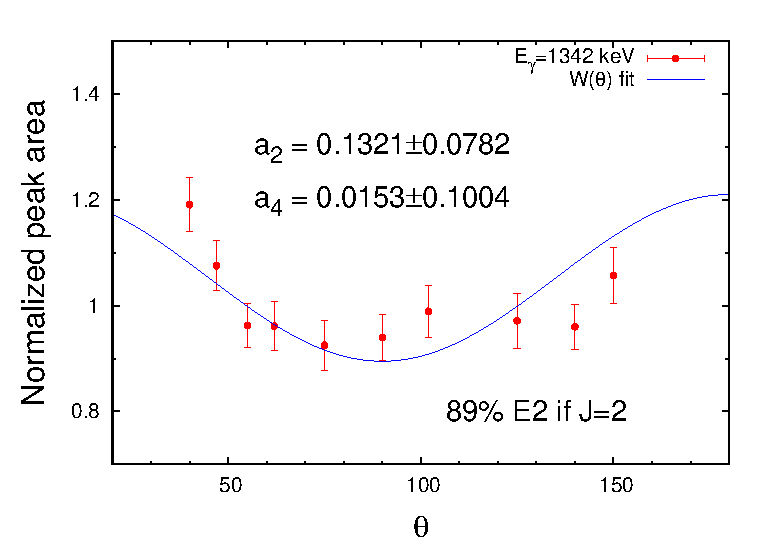
\includegraphics[width=0.999\textwidth]{figures/1342_AD.eps}
\caption{Measured angular distribution of 1342~keV $\gamma$ ray leaving the 2230~keV level, W($\theta$) fit is shown with a$_2$ and a$_4$ coefficients from the E$_n$=3.1~MeV angular distribution. \label{fig:1342_AD}}
\end{center}
\end{figure}

This begs the question, once again: where is the single-phonon $\beta$ vibration in $^{162}$Dy? If we take this state at 2230~keV as part of the $\beta\gamma$-vibration and with close to harmonic vibrations, the $\beta$ vibration \textit{should} be around E$_{\rm x}\approx$1350~keV; this is clearly not the case based on our lifetime measurements of the 0$^+_2$ band and its characterization as the K=0 $\gamma\gamma$-vibration. That being said, it is entirely possible that a strong $\beta$-vibration exists at either of the 0$^+$ excitations at 1814 or 1820~keV (or at the unobserved and elusive state at 774~keV). In the case of a $\beta$ vibration at $\sim$1800~keV, it would imply that the $\beta\gamma$ is fairly anharmonic, clocking in at $\sim$80\% of the expected two-phonon energy, which is reasonable, considering that the K$^\pi$=0$^+$ $\gamma\gamma$-vibration in $^{162}$Dy is $\sim$79\% harmonic (R$_{\frac{E_{\gamma\gamma}}{2E_\gamma}}\approx$0.79), and the K$^\pi$=4$^+$ $\gamma\gamma$-vibration is similarly anharmonic at R$_{\frac{E_{\gamma\gamma}}{2E_\gamma}}\approx$0.86. We strongly emphasize further study on the 0$^+$ states in $^{162}$Dy to find the collective $\beta$-vibration at 774, 1814, or 1820~keV (if the $\beta$-vibration even exists in this nucleus).

\begin{landscape}
\begin{figure}[t]
\begin{center}
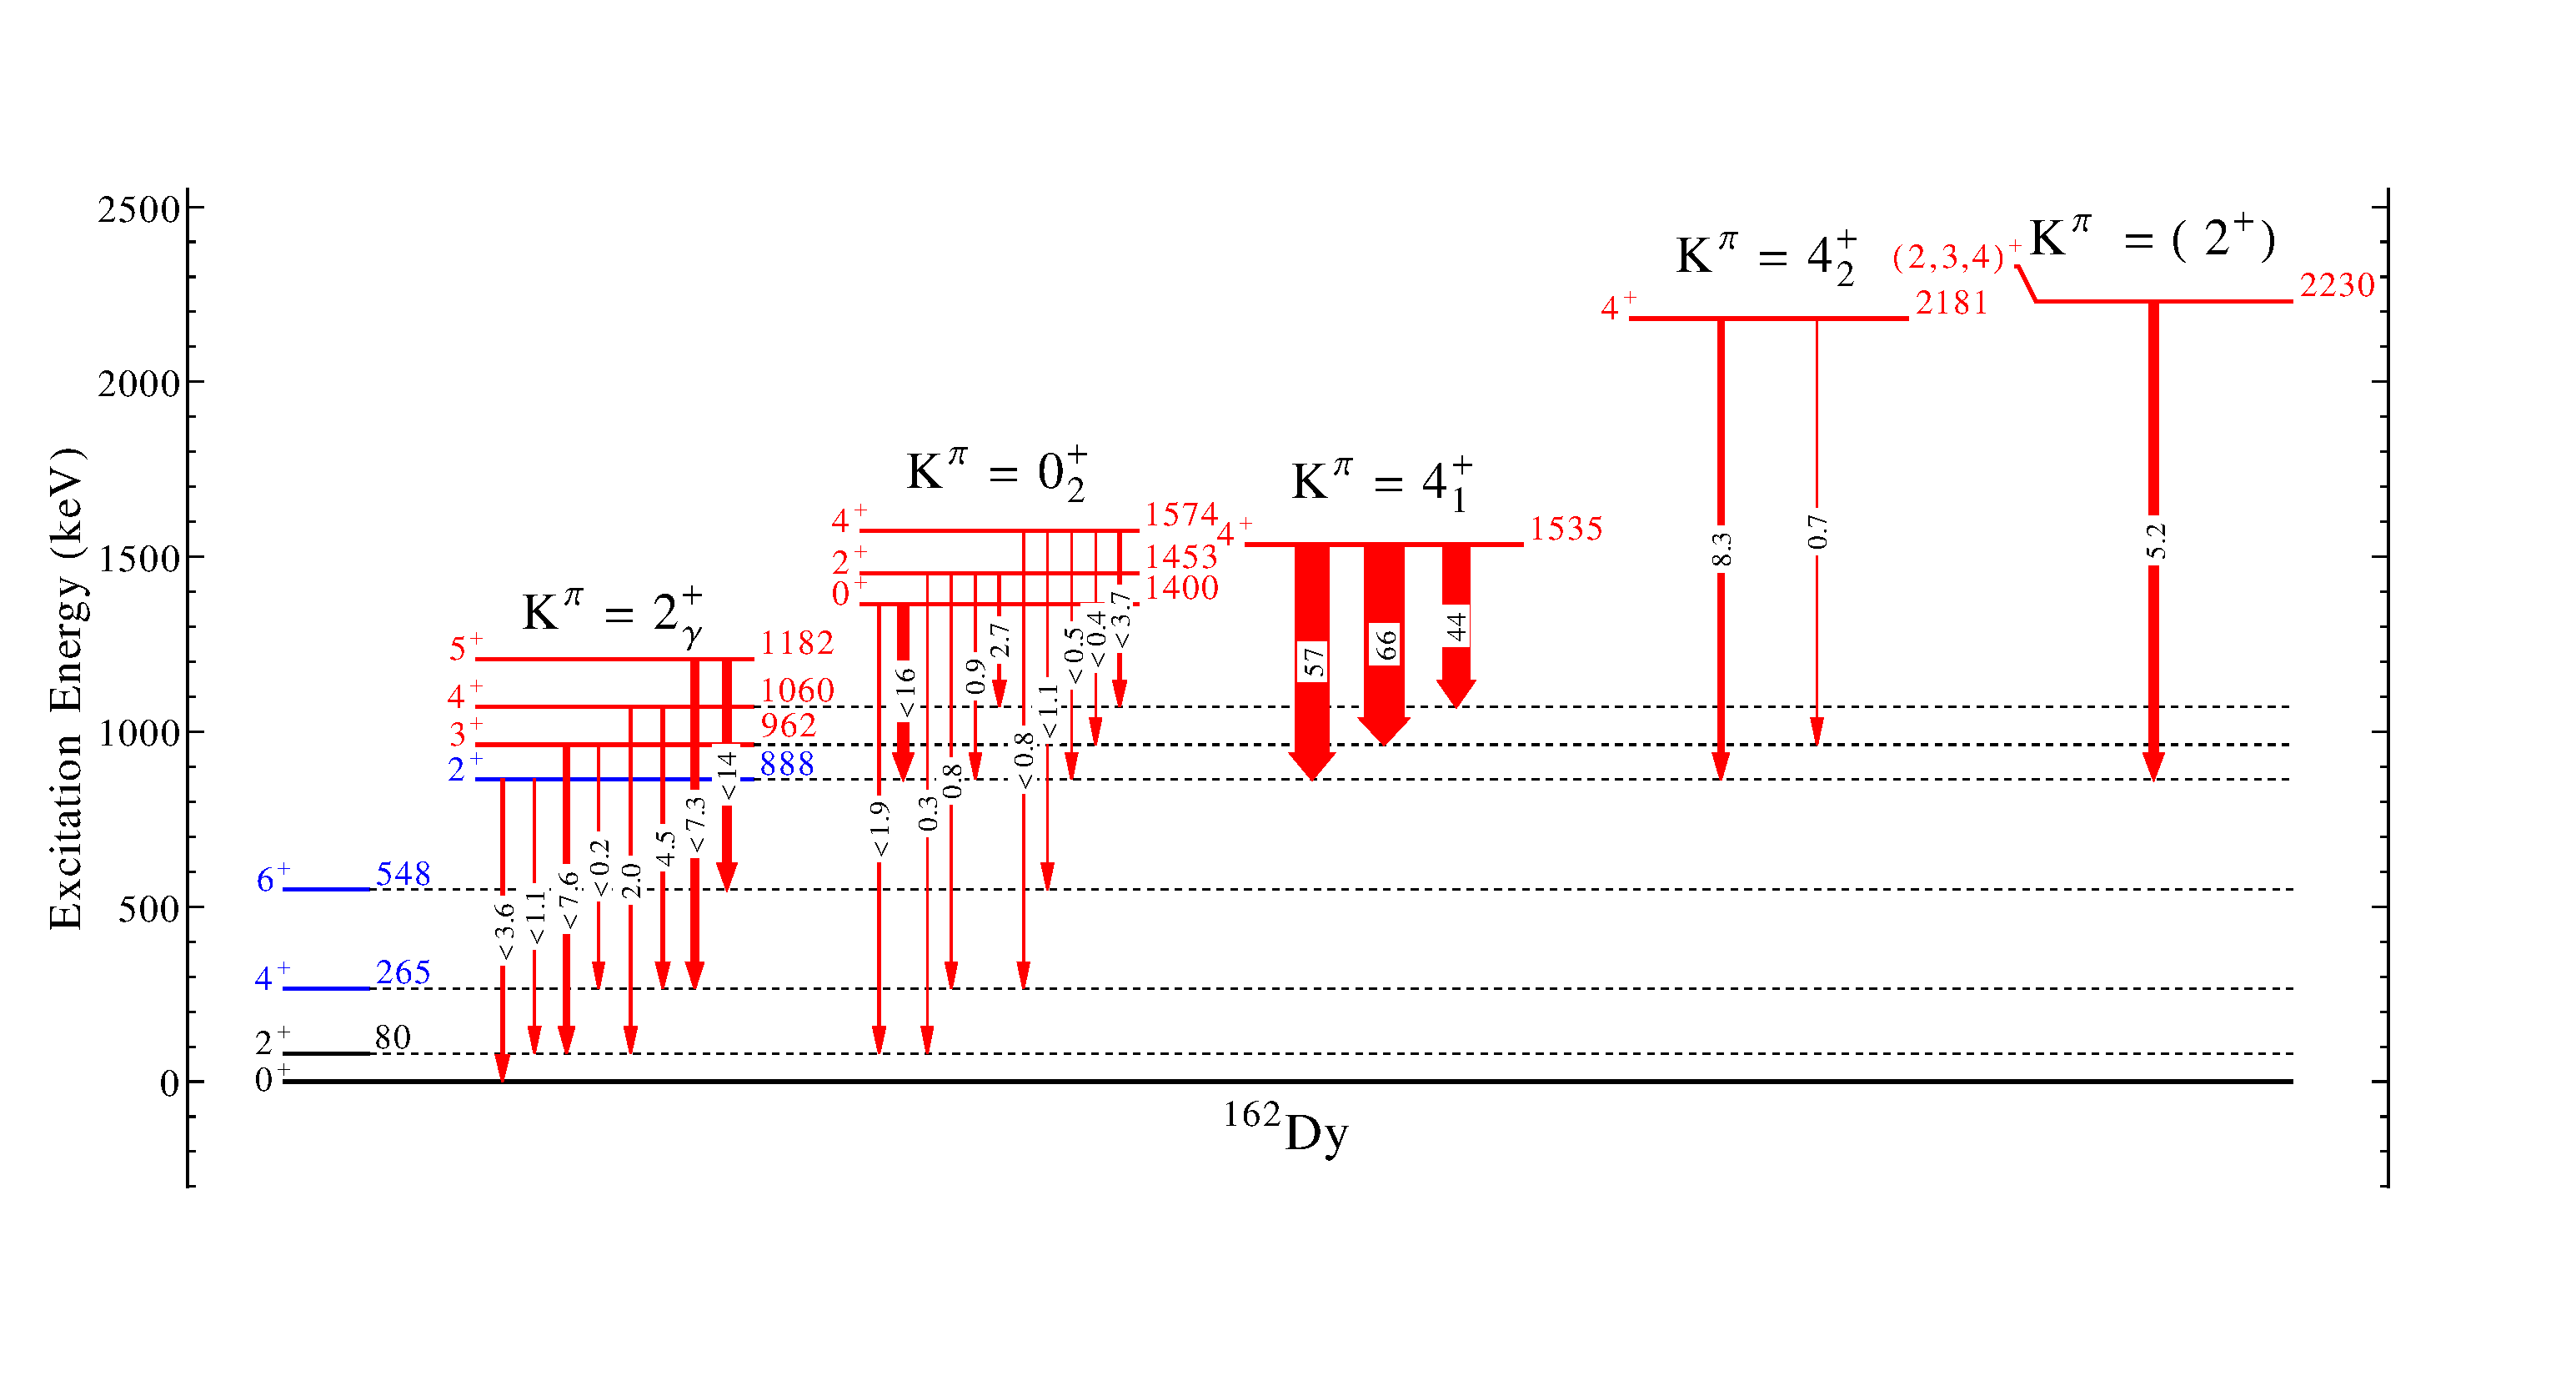
\includegraphics[height=0.85\textheight]{figures/162Dy_multiphonon042.pdf}
\caption{Level scheme showing all observed transitions from the lowest-lying 2$^+_\gamma$, 0$^+_2$, and 4$^+_1$ band with all interband (K$^\pi$=J$^+_i\rightarrow$K$^\pi$=2$^+_\gamma$) decays. Intensities for transitions to the $\gamma$-band are taken from \cite{Aprahamian200642}. Also shown is a tentative (2$^+$) state at 2230~keV with a strong decay to the 2$^+_\gamma$ band.
\label{fig:162Dy_multiphonon_042}}
\end{center}
\end{figure}
\end{landscape}

% \begin{center}
\begin{longtable}{l|l|l|l}
% \begin{table}[ht]
% \begin{tabular}{l|l|l|l}
% \begin{tabular}{ccc}
 \caption{OBSERVED/LITERATURE INTENSITIES (K$^\pi$=0$^+$,2$^+$,4$^+$): $^{162}$DY \label{tab:162Dy_multiphonon_intensities}}\\
E$_{lev}$ (keV) & E$_\gamma$ (keV) & I$_{\gamma,abs}$ (n,n$^\prime\gamma$) & I$_\gamma$ (lit.) \\ \hline\hline\endfirsthead 
 \caption[]{OBSERVED/LITERATURE INTENSITIES (K$^\pi$=0$^+$,2$^+$,4$^+$): $^{162}$DY}{Continued}\\
E$_{lev}$ (keV) & E$_\gamma$ (keV) & I$_{\gamma,abs}$ (n,n$^\prime\gamma$) & I$_\gamma$ (lit.) \\ \hline\hline\endhead 
  888.18(22) &  807.54(50)               &976.596(9.252)  & \\% 1.6
             &  888.18(50)               &887.460(7.953)  & \\ \hline% 1.6
  962.96(27) &  697.30(50)$^{[\oslash]}$ &166.366(2.981)  & \\% 1.6
             &  882.31(50)               &877.632(9.095)  & \\\hline% 1.6
 1061.05(29) &  795.35(50)               &213.256(1.374)  & \\% 1.6
             &  980.36(51)               &121.782(1.166)  & \\\hline% 1.6
 1182.88(26) &  634.24(61)               &  67.548(1.514) & \\%2.2 ->  67.548     1.514
             &  917.18(51)               & 214.971(2.635) & \\\hline%2.2 ->  214.971     2.635          
 1400.29(36) & 512.0(2)                  &  $[\dagger]$   & 11(5)* \cite{Zamfir_162Dy0_1999}\\
             & 1319.60(51)               & 163.971(1.238) & 133(3)* \cite{Zamfir_162Dy0_1999}\\ \hline%2.2
1453.50(30)  & 395.49 (10)               &  $[\dagger]$   & 0.18(2) \cite{Aprahamian200642}\\
             & 565.32 (12)               &  $[\dagger]$   & 0.37(6) \cite{Aprahamian200642}\\
             & 1187.81(51)               & 125.506(1.610) & 12.7(3) \cite{Aprahamian200642}\\ %2.2
             & 1372.80(51)               & 169.820(1.989) & 18.1(8) \cite{Aprahamian200642}\\ \hline%2.2
 1535.97(23) &  475.27(54)$^{[\otimes]}$& 53.276(3.388)  & 4.5(3) \cite{Aprahamian200642}\\ %2.2
             &  572.96(50)               & 90.678(1.588)  & 21.8(9) \cite{Aprahamian200642}\\  %2.2
             &  647.61(50)$^{[\oslash]}$ &141.966(2.084)  & 50.1(8) \cite{Aprahamian200642}\\ \hline %2.2
1574.34(29)  & 513.31 (2)                &  $[\dagger]$   & 0.51(3) \cite{Aprahamian200642}\\
             & 611.23 (5)                &  $[\dagger]$   & 0.12(2) \cite{Aprahamian200642}\\
             & 686.15 (6)                &  $[\dagger]$   & 0.29(8) \cite{Aprahamian200642}\\
             & 1025.84(58)$^{[\oslash]}$ &  25.251(0.916) & 5.0(2) \cite{Aprahamian200642}\\    %2.2
             & 1308.65(51)               & 135.879(1.997) & 24(2)  \cite{Aprahamian200642}\\  \hline %2.2
1666.01(33)  & 1585.35(51)               & 131.018(1.476) & \\  \hline %2.2
1728.31(20)  & 1462.70(51)$^{[\otimes]}$& 110.002(1.779) & 0.81(6) \cite{Govor_162Dy2002} \\   %2.2
             & 1647.64(51)               & 133.790(2.206) & 1.21(7) \cite{Govor_162Dy2002} \\   %2.2
             & 1728.29(53)               &  85.273(1.611) & 0.66(6) \cite{Govor_162Dy2002} \\  \hline %2.2
2128.02(33)  & 2047.34(61)               & 286.080(6.065) & \\ \hline  %3.1
 2180.69(53) &  1217.73(58)              &300.230(5.134)  & 1.13(24) \cite{Wu_2minus_2001}\\  %3.1
             &  1292.51(58)$^{[\otimes]}$&319.833(9.558) & 1.00     \cite{Wu_2minus_2001} \\ \hline %3.1 but on bkg
2189.65(52)  & 2109.10(50)               & 140.677(3.860) & \\ \hline  %3.1
 2231.06(38) & 1342.57(50)               &239.620(6.282)  & \\  \hline%3.1
2497.77(52)  & 2417.22(50)               & 116.520(4.933) & \\ \hline  %3.1
2655.83(33)  & 2575.28(53)               &  59.373(5.424) & \\  \hline %3.1
2802.04(61)  & 2721.48(55)               &  50.490(15.032)& \\ \hline  %3.1

% \end{tabular}


% \end{table}

\end{longtable}
\begin{flushleft}
\begin{singlespace}
Absolute intensities for $\gamma$-decays observed in (n,n$^\prime\gamma$) experiments. $[\dagger]$: $\gamma$ ray not observed, reporting literature intensity (\cite{Aprahamian200642,Govor_162Dy2002} gives absolute intensities, while \cite{Zamfir_162Dy0_1999,Wu_2minus_2001} report relative intensities).
\end{singlespace}
\end{flushleft}
% \end{center}

 \begin{table}
 \begin{center}
 \caption{ALAGA (K$^\pi$=0$^+$,2$^+$,4$^+$): $^{162}$DY \label{tab:162Dy_posparity_ALAGA}}

 \begin{tabular}{l c c|c}
 K$^\pi$ & $\frac{J_{K_i}\rightarrow J^\prime_{K_f}}{J_{K_i}\rightarrow J^{\prime\prime}_{K_f}}$ & Exp & CG$^2$ \\
 \hline
 \hline
 \underline{K$^\pi_i$=2$^+_\gamma$:} & $\frac{4^+\rightarrow4^+}{4^+\rightarrow2^+}$ & 2.3 & 2.9 \\
%                                      & $\frac{3^+\rightarrow4^+}{3^+\rightarrow2^+}$ & 0.1 & 0.4 \\ 
%                                      & $\frac{2^+\rightarrow2^+}{2^+\rightarrow0^+}$ & 0.3 & 1.4 \\
%                                      & $\frac{5^+\rightarrow6^+}{5^+\rightarrow4^+}$ & 1.9 & 0.6 \\
 \hline
 \underline{K$^\pi_i$=0$^+_2$:} & $\frac{2^+\rightarrow4^+}{2^+\rightarrow2^+}$ & 1.5 & 1.8 \\
                                & $\frac{4^+\rightarrow6^+}{4^+\rightarrow4^+}$ & 1.4 & 1.7 \\
                                & $\frac{2^+\rightarrow4^+_\gamma}{2^+\rightarrow2^+_\gamma}$ & 3.1 & 0.8 \\
                                & $\frac{4^+\rightarrow4^+_\gamma}{4^+\rightarrow2^+_\gamma}$ & 10 & 44 \\
                                & $\frac{4^+\rightarrow4^+_\gamma}{4^+\rightarrow3^+_\gamma}$ & 9.3 & 3.2 \\
                                & $\frac{4^+\rightarrow3^+_\gamma}{4^+\rightarrow2^+_\gamma}$ & 0.8 & 14 \\
                                                            \hline
 \underline{K$^\pi_i$=4$^+_1$:} & $\frac{4^+\rightarrow4^+}{4^+\rightarrow3^+}$ & 0.5$^{[\star]}$ (0.2) & 0.4 \\     
                                & $\frac{4^+\rightarrow4^+}{4^+\rightarrow2^+}$ & 0.8$^{[\star]}$ (0.2) & 0.2 \\ \hline
 \underline{K$^\pi_i$=4$^+_2$:} & $\frac{4^+\rightarrow3^+}{4^+\rightarrow2^+}$ & 0.1 & 0.6 \\                               
 \end{tabular}
 \end{center}
Alaga rule comparisons of measured B(E2) strengths for the K$^\pi$=2$^+_\gamma$, 0$^+_2$, and 4$^+_1$ band in $^{162}$Dy. $^{[\star]}$: Alaga comparison shown in parentheses uses literature intensities to calculate B(E2) strengths.
 \end{table}

\begin{table}
\begin{center}
\caption{B(E2) RATIOS (K$^\pi$=0$^+$,2$^+$,4$^+$): $^{162}$DY \label{tab:0_2_BE2ratios}}

\begin{tabular}{ccc}
K & $\frac{J_i\rightarrow J_f}{J_i\rightarrow J_f}$ & $\frac{B(E2\rightarrow\gamma)}{B(E2\rightarrow g.s.)}$ \\ \hline \hline
\underline{K$^\pi$=0$^+_2$:}& $\frac{0^+\rightarrow2^+_\gamma}{0^+\rightarrow2^+_{g.s.}}$ & 8.4 \\
& $\frac{2^+\rightarrow2^+_\gamma}{2^+\rightarrow2^+_{g.s.}}$ & 3.0 \\
& $\frac{2^+\rightarrow4^+_\gamma}{2^+\rightarrow4^+_{g.s.}}$ & 3.4 \\
& $\frac{4^+\rightarrow4^+_\gamma}{4^+\rightarrow4^+_{g.s.}}$ & 4.6 \\
\end{tabular}
\end{center}
Ratios of B(E2) probabilities of the transitions to the $\gamma$-band over the ground state band transitions, highlighting an enhancement or preference of decay to the K$^\pi$=2$^+\gamma$-band.
\end{table}

%%%%%%%%%%%%%%%%%%%%%%%%





% \begin{figure}[t]
% \begin{center}
% 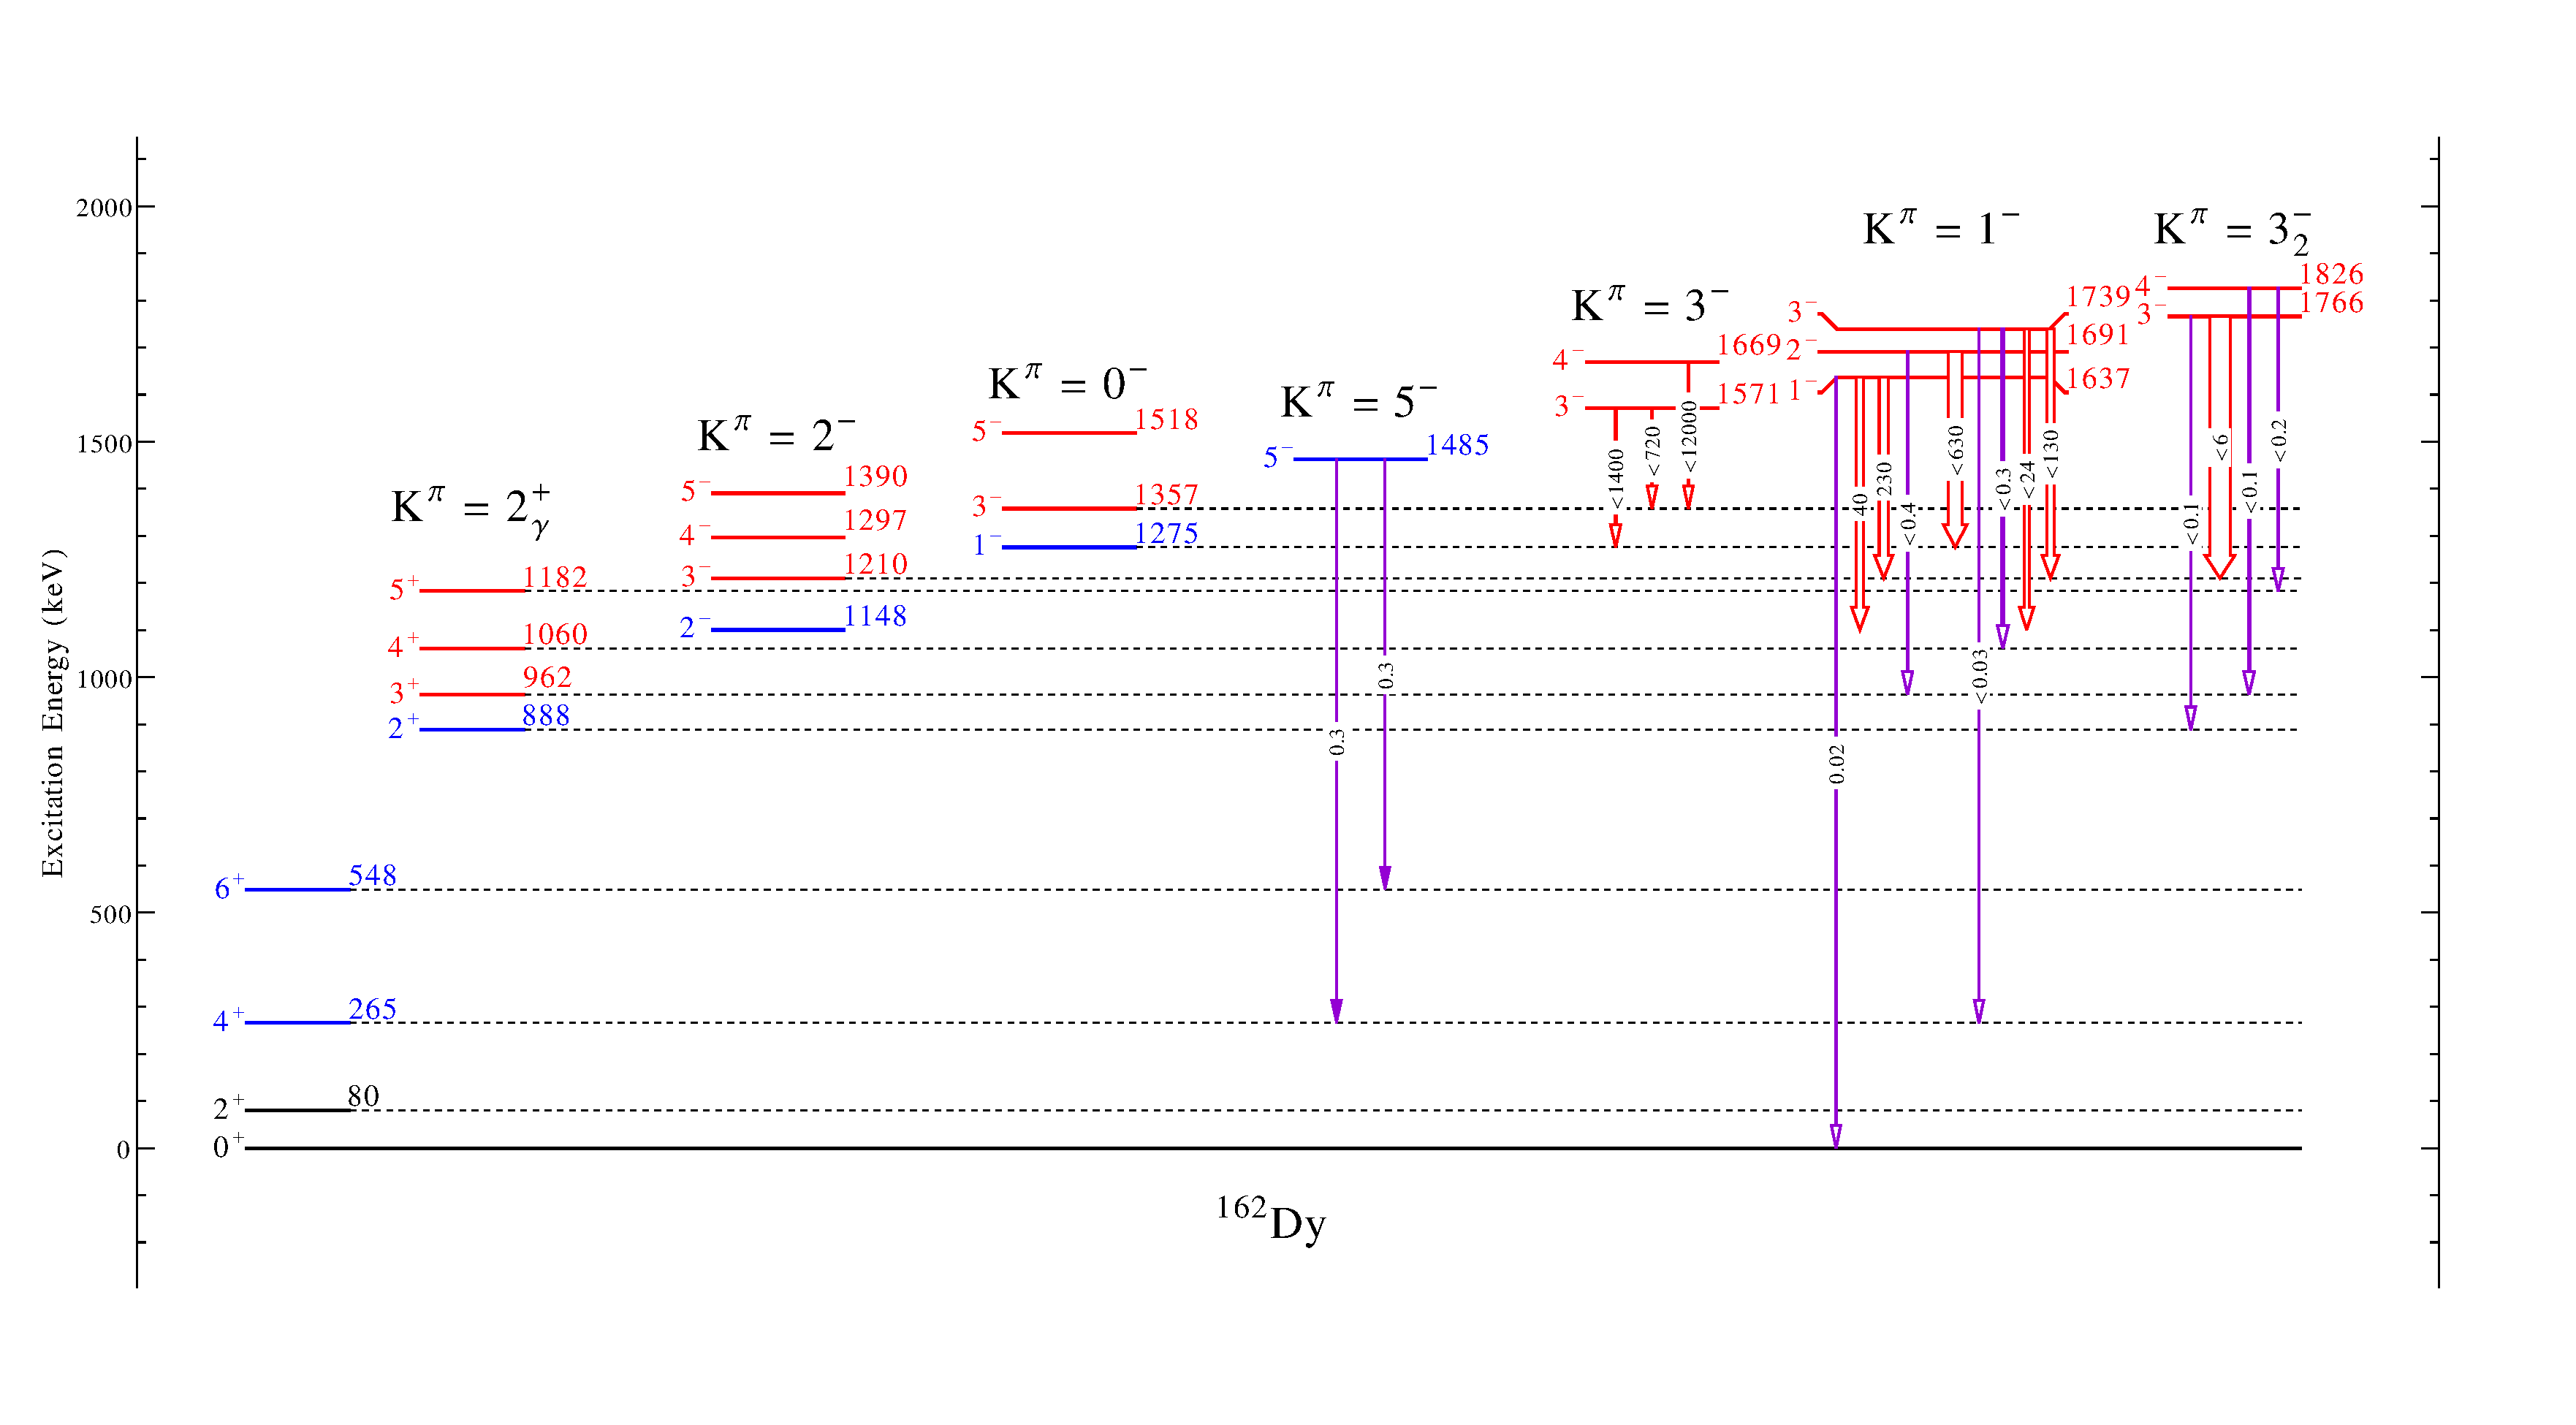
\includegraphics[width=0.95\textwidth]{162Dy_otherNeg.pdf}
% \caption{Higher-lying negative parity bands (K$^\pi$ = 5$^-$, 3$^-_2$, 4$^-$, \& 2$^-_2$) in $^{162}$Dy with drawn transition widths proportional to the calculated reduced transition probabilities. Here, B(E2) measurements are colored red, with B(E1) values in violet. \label{fig:162Dy_otherNeg}}
% \end{center}
% \end{figure}

% \begin{figure}[t]
% \begin{center}
% 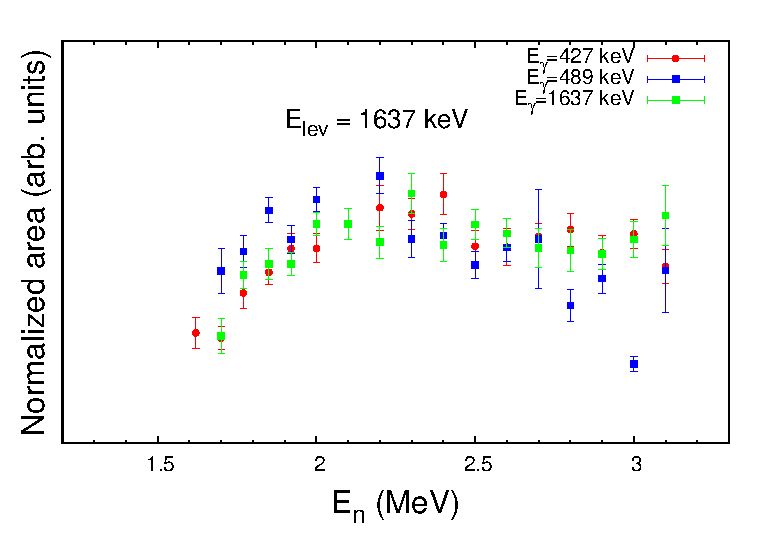
\includegraphics[width=0.95\textwidth]{162Dy_1minus_ExF.eps}
% \caption{Excitation function measurements for $\gamma$ rays leaving the bandhead of the 1$^-$ band.  \label{fig:162Dy_1minus_ExF}}
% \end{center}
% \end{figure}


% \subsection{Other Lifetime Measurements}
% 
% Our discrepancy in lifetime measurement with respect to the literature value for the K$^\pi$=5$^-$ bandhead is striking, much like the case for the E$_{\rm x}$=1148~keV level, yet we repeat the same assertions made in the previous section. The two de-exciting $\gamma$-rays exhibit a rather unambiguous placement in the level scheme from our measurement of the excitation function (both E$_\gamma$=937 \& 1220~keV $\gamma$ rays match qualitative shape and have the same threshold, consistent with a 5$^-$ state at 1485~keV), and show well-defined Doppler energy-shifts that correspond to a lifetime of 450~fs, compared to the literature value of 1.92~ns \cite{Honig_5minus1969}. We contest this lifetime measurement via delayed-coincidence from the $\beta$-decay of $^{162m}$Ho, from our unambiguous placement of de-exciting $\gamma$ rays in the level scheme, accurate branching ratios in comparison to literature intensities, and well-behaved DSAM shifts. In scrutinization of the literature, it is found that the 1.92~ns lifetime measurement by \cite{Honig_5minus1969} is explicitly placed for the nearby 1490~keV state, and very little discussion is made on the delayed-coincidence measurements made in \cite{CHARVET_162Dy5minus}. It is not entirely unreasonable that the measured lifetime in \cite{Honig_5minus1969,CHARVET_162Dy5minus} are instead seeing this nearby state at 1490~keV. This 7$^+$ state de-excites via a very similar energy (940~keV versus 937~keV) $\gamma$ ray, and is populated via first-forbidden Fermi-type $\beta$-decay, in contrast to the preferred Gamov-Teller decay to the 5$^-$ at 1485~keV. The current status/insight of this K$^\pi$=5$^-$ band is of a two-quasiparticle origin \cite{Aprahamian200642}, where we can verify this interpretation with our (albeit slightly inflated at $\sim$0.3~mWu) weak E1 transition strengths to the ground state.
% 
% \begin{figure}[ht]
% \begin{center}
% 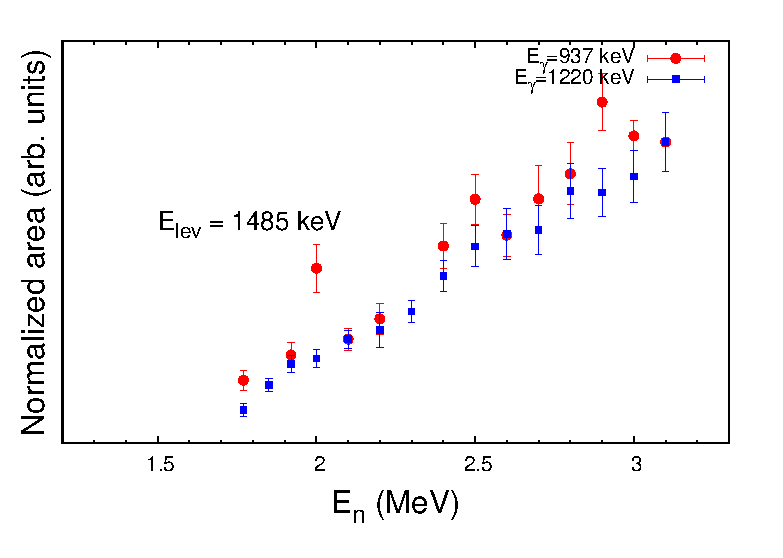
\includegraphics[width=0.75\textwidth]{937_ExF.eps}\\
% 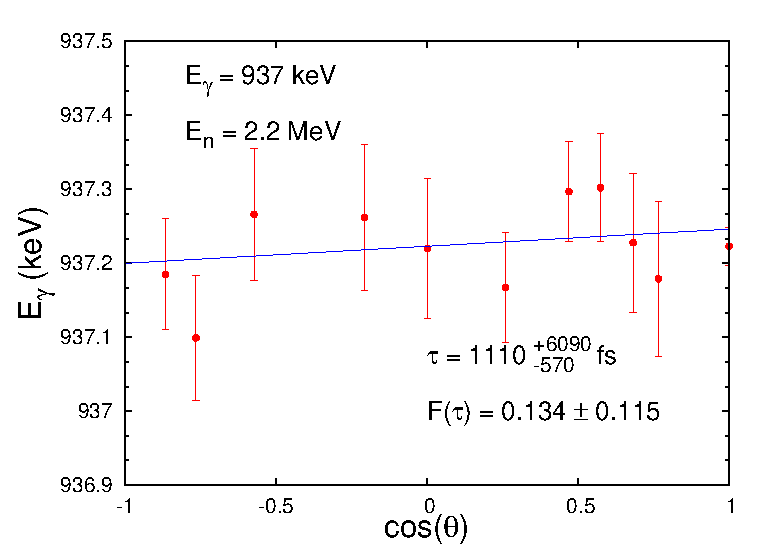
\includegraphics[width=0.49\textwidth]{937_DSAM.eps}
% 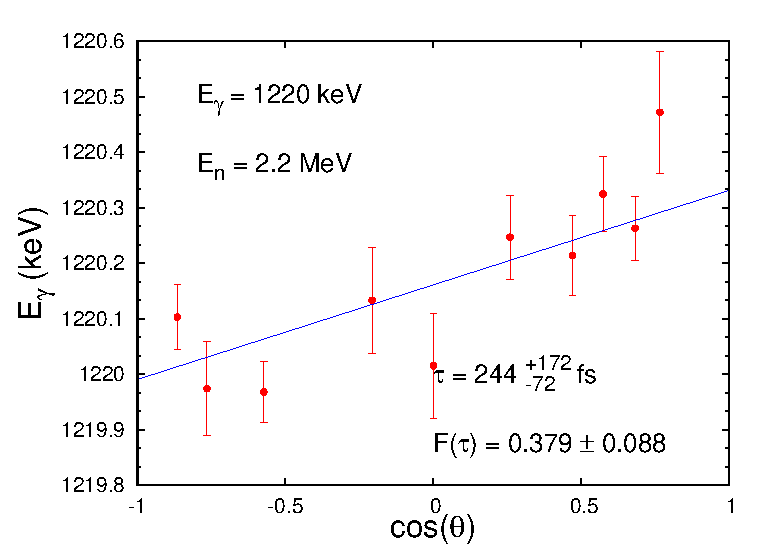
\includegraphics[width=0.49\textwidth]{1220_DSAM.eps}
% \caption{E$_\gamma$=937 \& 1220~keV (de-excitations from the E$_{\rm x}$=1485~keV level) Doppler shifts and overlaid excitation functions (color online). The excitation function (in blue) for the 1220~keV $\gamma$ ray is scaled by a factor of 0.291. \label{fig:1485_DSAM_EXF}}
% \end{center}
% \end{figure}
% 
% Assertions from IBM considerations with the inclusion of \textit{p} and \textit{f} bosons imply that the structure of the lowest-lying negative parity bands may not be of purely collective nature  \cite{Aprahamian200642, Iachello_Arima_IBM}, where the traditional picture of octupole collectivity in well-deformed nuclei exists with the initial, lowest-lying and fragmented quartet of states of K$^\pi$=0$^-$, 1$^-$, 2$^-$, \& 3$^-$. However, the current ordering of negative parity bands in $^{162}$Dy is difficult (read: impossible) to predict with modern models \cite{Aprahamian200642}. We have measured lifetimes for a few other of the lowest-lying set of states in $^{162}$Dy, where we provide individual discussion on our measurements.
% 
% Absolute intensities from $\gamma$ rays depopulating the K$^\pi$=3$^-$ band at 1570~keV show an obvious preference to the previously established 0$^-$ octupole band \cite{Aprahamian200642} in the literature, where we do not observe the full 3$^-\rightarrow$\textit{g.s.} transitions due to the low branching ratios listed. Shallow shifts in the DSAM fitting only gives a lower limit to the lifetime of the 3$^-$ bandhead of $>$3050~fs, where, in contrast, we get good lifetime resolution on the 4$^-$ member; this creates a somewhat murky picture for any interpretation of the K$^\pi$=3$^-$ band. The E$_\gamma$=311~keV de-excitation from the 4$^-$ member is overwhelmingly E2 radiation, based on our measurement of a mixing ratio of -6.9$^{+1.6}_{-2.2}$ ($\sim$98\% E2), but the very large (potentially) E2 transition probabilities that de-excite the bandhead are impressive, even in the face of heavy M1 mixing for the 212~keV $\gamma$ ray that leaves the bandhead at 1570~keV. That being said, we yet again encounter some of the limitations behind the Doppler Shift Attenuation Method, in that lower energy $\gamma$ rays ($<$500~keV) are easily attenuated by the sample size and may not exhibit reliable energy shifts. Further investigation of this level lifetime with another measurement technique (Coulomb excitation, `plunger' method with RDDM, etc) is desired to more confidently understand the transition probabilities here, as the lifetimes measured in our campaign of experiments seem to be fairly unreliable. Whether this band is some higher collective behavior on top of the existing octupole vibration or if it is even part of the 0$^-$, 1$^-$, 2$^-$, 3$^-$ quartet is still an open question, however, the preference of decay to the lower-lying octupole band (K$^\pi$=0$^-$ band) should not be understated.
% % K=3- band could be a double octupole, with strong preference to decay to the k=0-, really, this breaks the notion that the lowest-lying neg parities are the fragmented octupole
% 
% 
% The K$^\pi$=1$^-$ band at 1637~keV provides some of the least consistent and reliable results from our experimental campaign to measure lifetimes in $^{162}$Dy. Starting with the bandhead, the only $\gamma$ ray to attribute to the lifetime measurement is the de-excitation of E$_\gamma$=1637~keV. The questionability of this $\gamma$-ray placement is an issue, in that (n,$\gamma$) reactions by \cite{Aprahamian200642} do not observe it, yet other (n,n$^\prime\gamma$) experiments do. Nevertheless, the other two observed decays cannot be used because the 427~keV line is coincident with a background line, and as such, the extracted F($\tau$) is not reliable; the 489~keV $\gamma$ provides an alternate discussion on its exclusion from the level lifetime. First, the relative intensity of the radiation does not fall in line with the other de-excitations according to the literature, and second, the extracted F($\tau$) from the 427~keV line varies wildly (by more than 2$\sigma$) from the 1637~keV line, and lastly, the excitation function(s) (Figure \ref{fig:162Dy_ExF1637}) for de-excitations out of the bandhead show an inconclusively similar pattern, qualitatively. These reasons are indicative of a bad placement of this decay in the level scheme, and is indicated by parentheses in Table [REF]. Further proof of the 489~keV $\gamma$ ray being a contaminant can be seen in the nonconvergence of a multipole mixing fraction (ranging from 33-91\% E2, with a large $\chi^2$ value on the angular distribution).
% 
% \begin{figure}[ht]
% \begin{center}
% 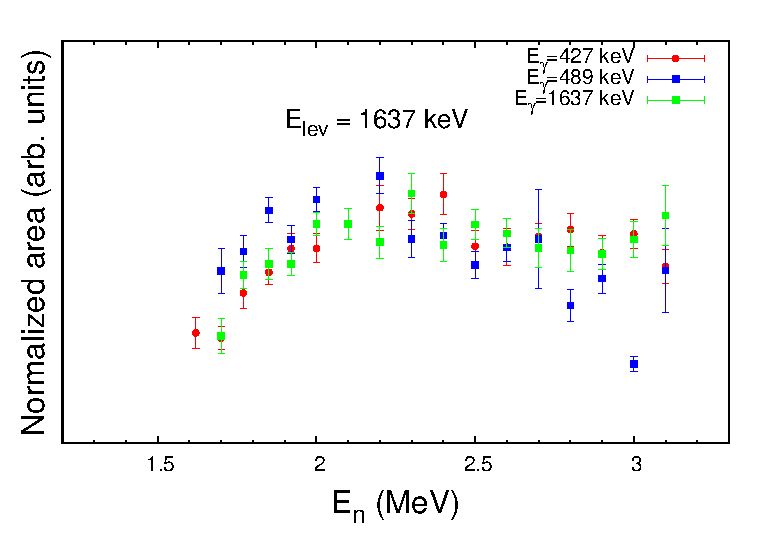
\includegraphics[width=0.97\textwidth]{162Dy_1minus_ExF.eps}
% \end{center}
% \caption{Excitation functions for the decays leaving the E$_{\rm x}$=1637~keV state. (color online)\label{fig:162Dy_ExF1637}}
% \end{figure}
% 
% The 2$^-$ member of the band also yields some less than stellar resolution on the nuclear lifetime. With two decays observed at intermediate energies (but still below 1~MeV), we are only able to rely on the 728~keV $\gamma$ ray to measure the lifetime, as the 416~keV decay lies on top of a background. The resulting lifetime limit of $>$1000~fs extracted from the Doppler Shift is not reliable, with F($\tau$) being consistent with zero within 1$\sigma$ uncertainty. Since the 416~keV $\gamma$ ray is coincident with a background, a reliable multipole mixing fraction cannot be extracted from the angular distributions, as we do not know the distribution of the background as a function of angle. As such, the deduced transition probabilities should not be taken without careful attention and heavy skepticism. Interband B(E2) strengths of 630~W.u. are unprecedented in \textit{any} nuclear transition, flagging a clear departure from a consistent measurement of the lifetime.
% 
% The 3$^-$ member offers a slight tangent from the echoed rhetoric in the 1$^-$ band, but still does not behave well. The extracted average level F($\tau$) value is just over 1$\sigma$ deviant from 0, giving both a) a borderline unreliable lifetime extraction, and b) an extremely low magnitude lower limit of $>$740~fs, which does not offer vast insight into the collectivity of the band. In this sea of delinquent behavior, the branching ratios for the 3$^-$ state of the 1$^-$ band agree well with literature \cite{Aprahamian200642}, but the multipole mixing fraction for the 529~keV $\gamma$ is deviant from literature ($\sim$50\% mixed, vs $>$99\% M1 in literature). Again, the resulting B($\pi\ell$) strengths for decays out of the 3$^-$ state are vast upper limits from our experiments. 

%do an ExF for the 1739 state here too




% we observe remarkably strong B(E2)s to the 2$^-$ band, even considering the large uncertainties and heavy E2/M1 mixing to the bandhead of the 2$^-$ band. The full energy de-excitation to the ground state exhibits a very non-collective E1 transition, immediately pointing away from a single-octupole picture. The 1691~keV state follows in line with the bandhead, with a strong B(E2) to the 2$^-$ band with high M1-mixing and a somewhat suppressed transition probability to ground state. Mixing information was not extracted for the 416~keV $\gamma$ ray to the 0$^-$ octupole band, so the quoted B(E2) value in Table \ref{tab:162Dy_negparity_low} is essentially an upper limit. Yet again, in the 3$^-$ member of the band, we observe strong E2 radiation to the 2$^-$ band (the 529~keV $\gamma$ ray is $\sim$100\% M1 radiation), with suppression of B(E1)s to the $\gamma$ and ground state band. Qualitatively, this suggests some strong quadrupole collectivity built on top of the 2$^-$ band in $^{162}$Dy; this deduction and decay pattern is in stark contrast to the simple picture of octupole collectivity in deformed nuclei, where the lowest quartet of negative parity states arise from the single $\lambda$=3 phonon fragmentation. Nearby rare-earth nuclei ($^{168}$Er) display strong E3 transition probabilities, with suppressed intraband B(E1)s [REFS], making $^{162}$Dy an anomaly in this sense. From our measurement of lifetimes and $\gamma$-ray spectroscopy, the question on the existence of this traditional picture of octupole collectivity seems tentative, with the existence of strong electric dipole transitions to the $\gamma$-vibrational band and to lower-lying negative parity states.


% \subsection{Higher Lying K$^\pi$=5$^-$, 3$^-_2$, 2$^-_2$ Bands}


% Decays from the second K$^\pi$=3$^-$ band have the potential for some interesting structure effects, with the extremely preferential branching ratios to the $\gamma$-band and the K$^\pi$=2$^-$ band. However, our measurements of the second K$^\pi$=3$^-$ band's lifetimes cannot reveal any insight to the octupole collectivity in these levels. F($\tau$) values for the bandhead at 1766~keV fail to display any definite shift in energy, in fact, having a negative (completely unphysical) value with a very large error. The unreliable lifetime reported in this work is simply the lower limit where F($\tau$) is the most positive, at a value of 0.044, but this extracted lifetime of 3400~fs should not be taken with any amount of confidence. The same can be said about the 4$^-$ member at 1826~keV: the extracted F($\tau$) is \textit{very} consistent with zero, as the only available transition to $\gamma$-band at 863~keV transition energy gives an appreciably nonzero shift (though not by much). Again, the lower limit of the lifetime is taken at the very edge of what F($\tau$) can be (at a value of 2400~fs).The statistical model employed ({\tt CINDY} \cite{SHELDON197399}) to calculate multipole mixing fractions was able to converge on a value for the mixing ratio from the 556~keV $\gamma$ ray's angular distribution, however. In the case of mostly E2 radiation and the lowest possible lifetime, the alarmingly large B(E2)$\sim$6~Wu to the 2$^-$ band could indicate some collectivity on top of the K$^\pi$=2$^-$ octupole band, based solely on the decay pattern, but nothing concrete can be said, barring a reliable measurement of the actual lifetime of the states in the band.

%REMOVE THIS SECTIOn
% The measurement of the single lifetime limit for the bandhead of the 4$^-$ is taken from the only de-excitation observed in a  E$_\gamma$=327~keV decay to the K$^\pi$=4$^+$ bandhead. Negative parity lifetimes were measured using the GRID technique by Aprahamian (unpublished work); the range of lifetimes measured in that experiment for the 1862~keV level are in excellent agreement with our limit (1580-2860~fs). (This same argument also applies to our measurement of the lifetime for the 5$^-$ state at 1485~keV, which was given an upper limit of 2910~fs from the Doppler broadening technique.) Using this range of lifetimes from GRID, we are presented with a much clearer picture on the collectivity of this state at 3.3-5.9~mWu strength for the decay to the 4$^+$ band. This rather enhanced B(E1) suggests the idea that there could be some definite octupole collectivity built on top of the K$^\pi$=4$^+$ band. 
%Remove this section

% 
% \begin{figure}[ht]
% \begin{center}
% 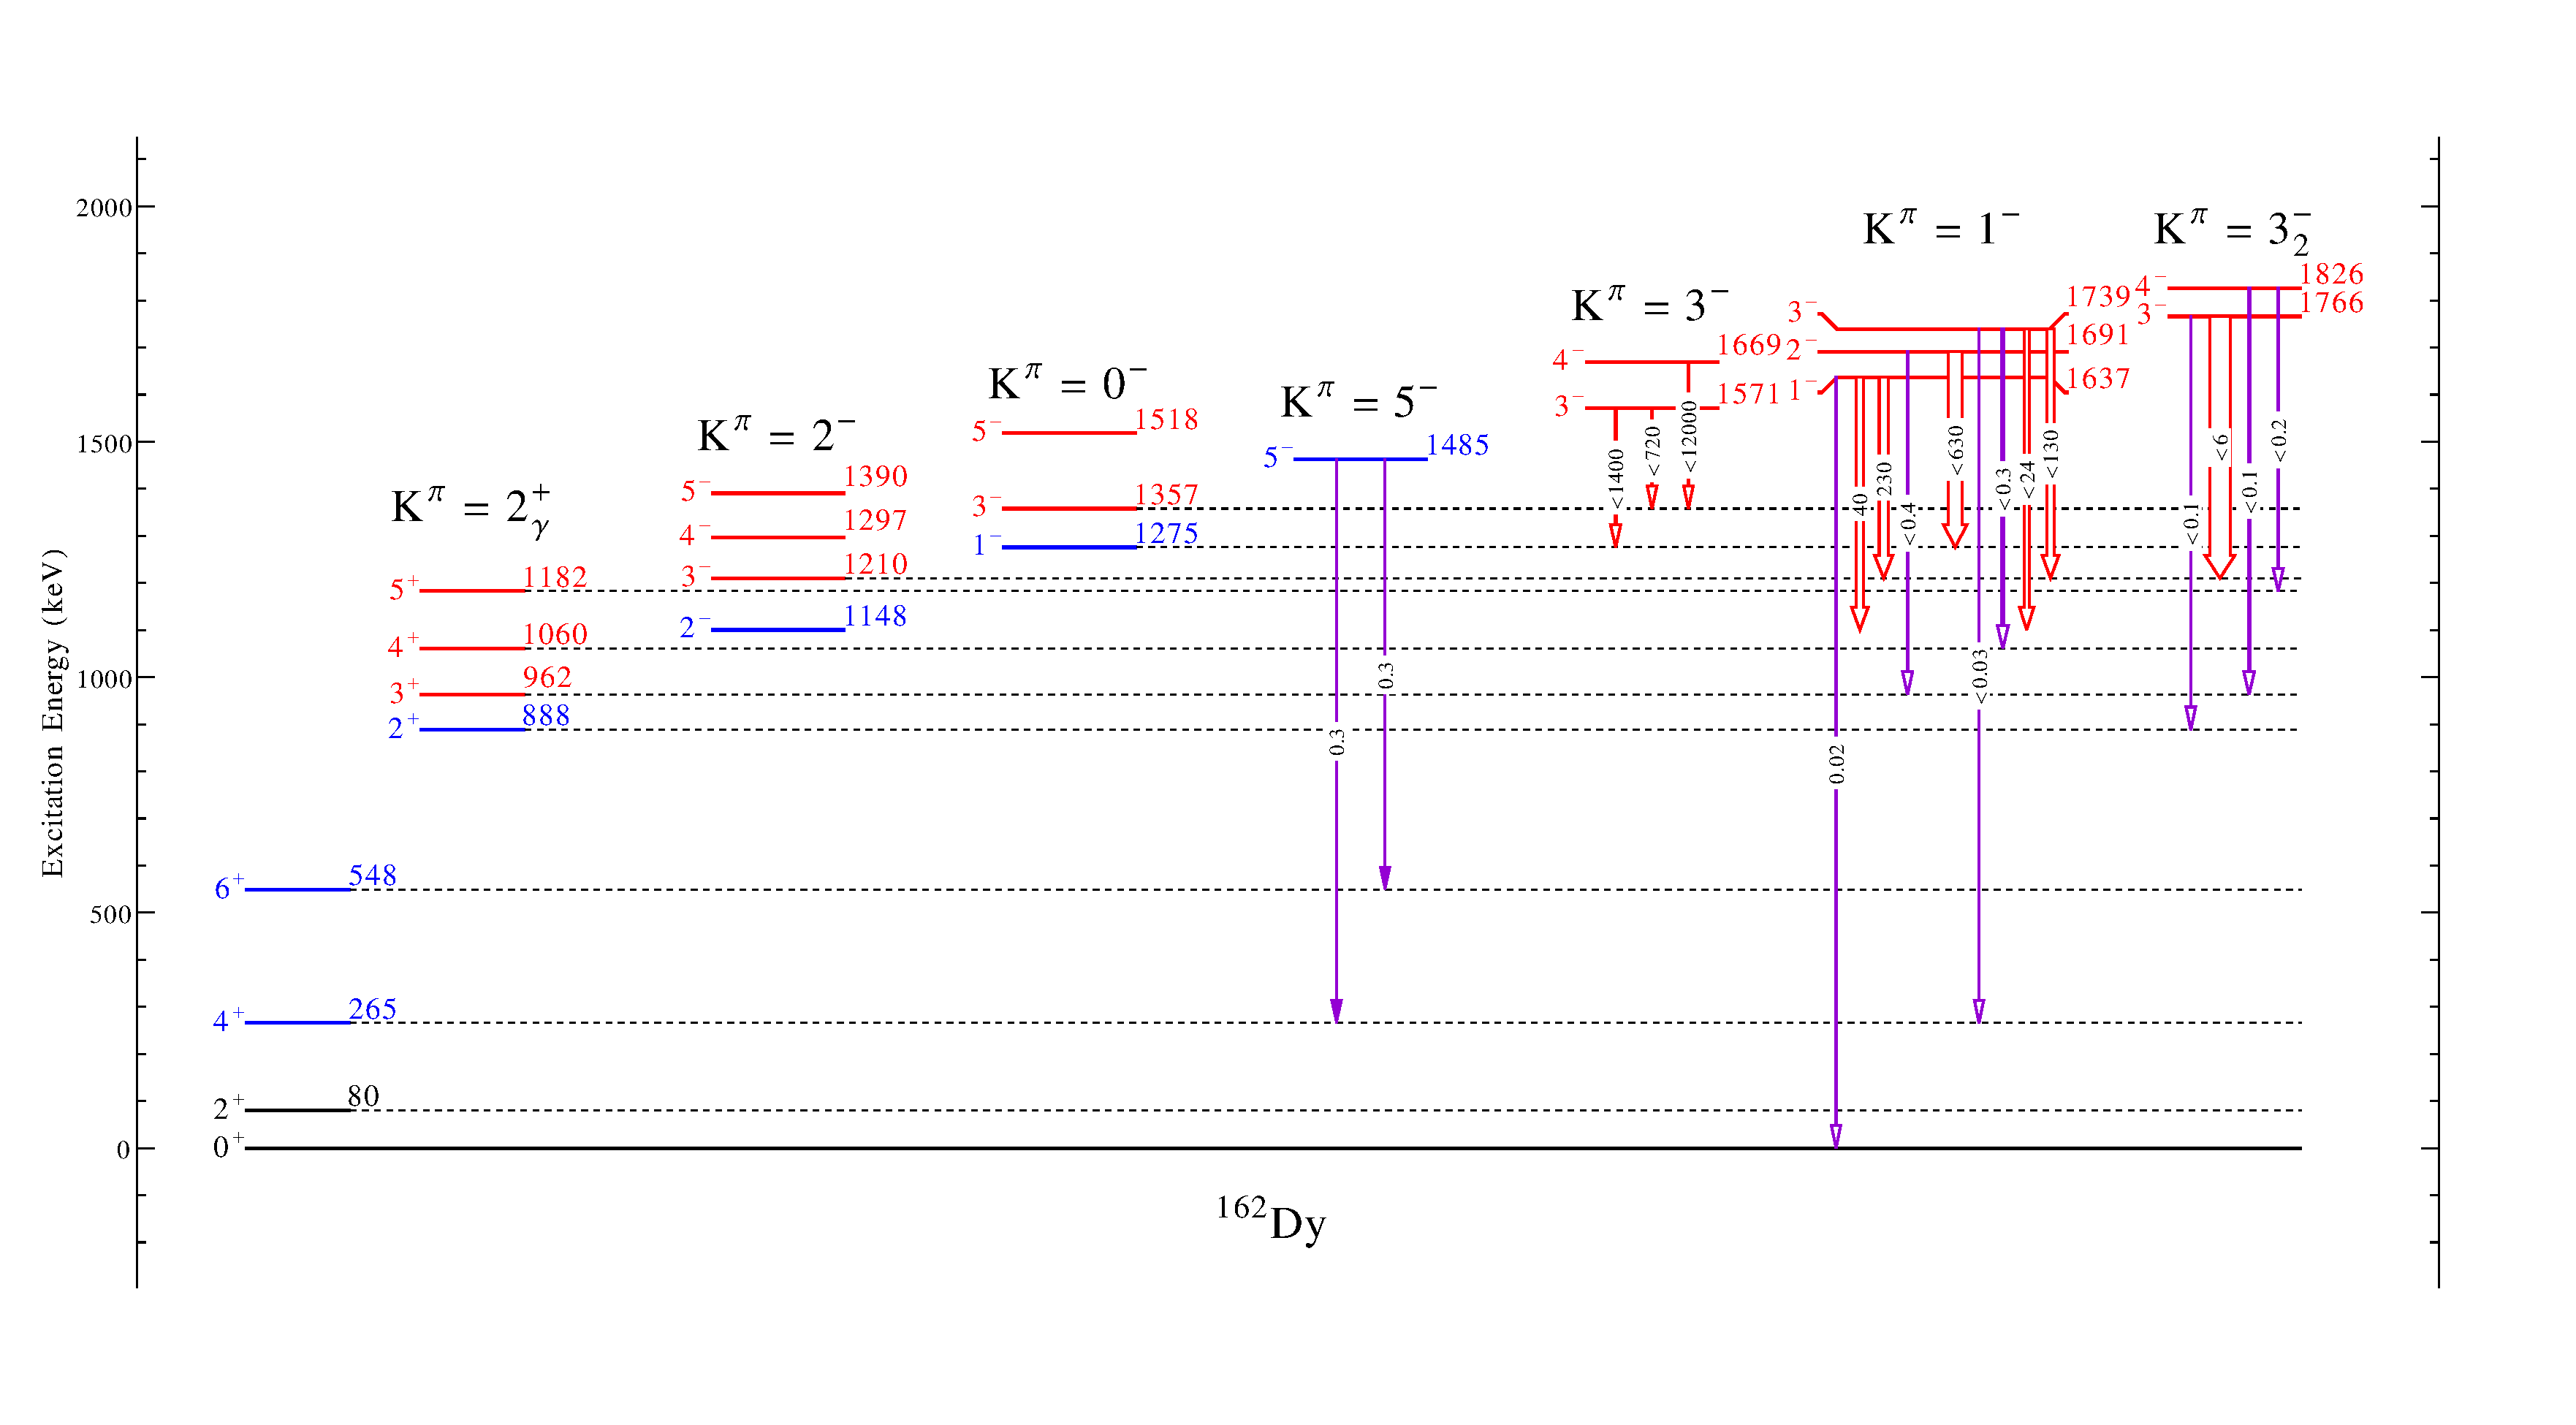
\includegraphics[width=0.98\textwidth]{162Dy_otherNeg.pdf}
% \caption{Observed $\gamma$-decays from higher lying K$^\pi$=5$^-$, 3$^-$, 1$^-$, 3$^-_2$ bands in $^{162}$Dy. Transition strengths are proportional in width, with E2 transitions in red and E1 transitions in violet (color online). \label{fig:162Dy_highbands}}
% \end{center}
% \end{figure}
